\documentclass[12pt]{report}
\usepackage[a4paper]{geometry}
\usepackage{amsmath, caption, cite, comment, graphicx, multirow, subcaption, url, float, verbatim}
\usepackage{float}
\graphicspath{ {images/} }
\begin{document}
\title{Restaurant Recommendation Based On MYSQL Database}
\author{Anjana Tiha\\
Department of Computer Science\\
University of Memphis, Memphis, TN\\
Email: atiha@memphis.edu\\\\
Supervised by: Professor Deepak Venugopal\\\\\\}
\maketitle
\section*{Introduction}
This report is aimed at providing details on restaurant recommendation system using relational database. This project is part of graduate course Database Systems in Computer Science program of University of Memphis. 
The database was developed with following concepts:
\begin{itemize}
\item Users can be identified by their email-id. Other information stored for a user includes
name, date of birth and address. Each user has a star rating (1-5) indicating trustworthiness.
\item A user may choose to follow other users.
\item Each user reviews one or more restaurants.
\item A review contains scores for the following items: Ambiance, Food Quality, Service,
Price and Overall Experience. Each score is on a discrete scale of 1 - 5 (5 denoting the
largest score). Optional free text comments are also saved.
\item Each restaurant has a name and address. The same restaurant name can have multiple
addresses. A restaurant belongs to exactly one of the following types: Ethnic, Fast
food, Fast casual, Casual dining, Family style or Fine dining.
\item A restaurant can serve multiple cuisines. Each user likes one or more cuisines.
\item A restaurant accepts coupons. A coupon contains a coupon-code which is unique to
a specific restaurant. The discount percentage and a specific date that the coupon is
valid is stored. Users can have multiple coupons.
\end{itemize}
This   The project was developed using MySQL, Python, Django web framework and Bootstrap. First we developed ER diagram. Then mapped them to relational table. Wrote SQl query for database creation, table creation and data insertion. 
\newpage
\section*{Database design}
\begin{figure}[H]
\begin{center}
\caption{Mapping the ER (or EER) model to a relational model}
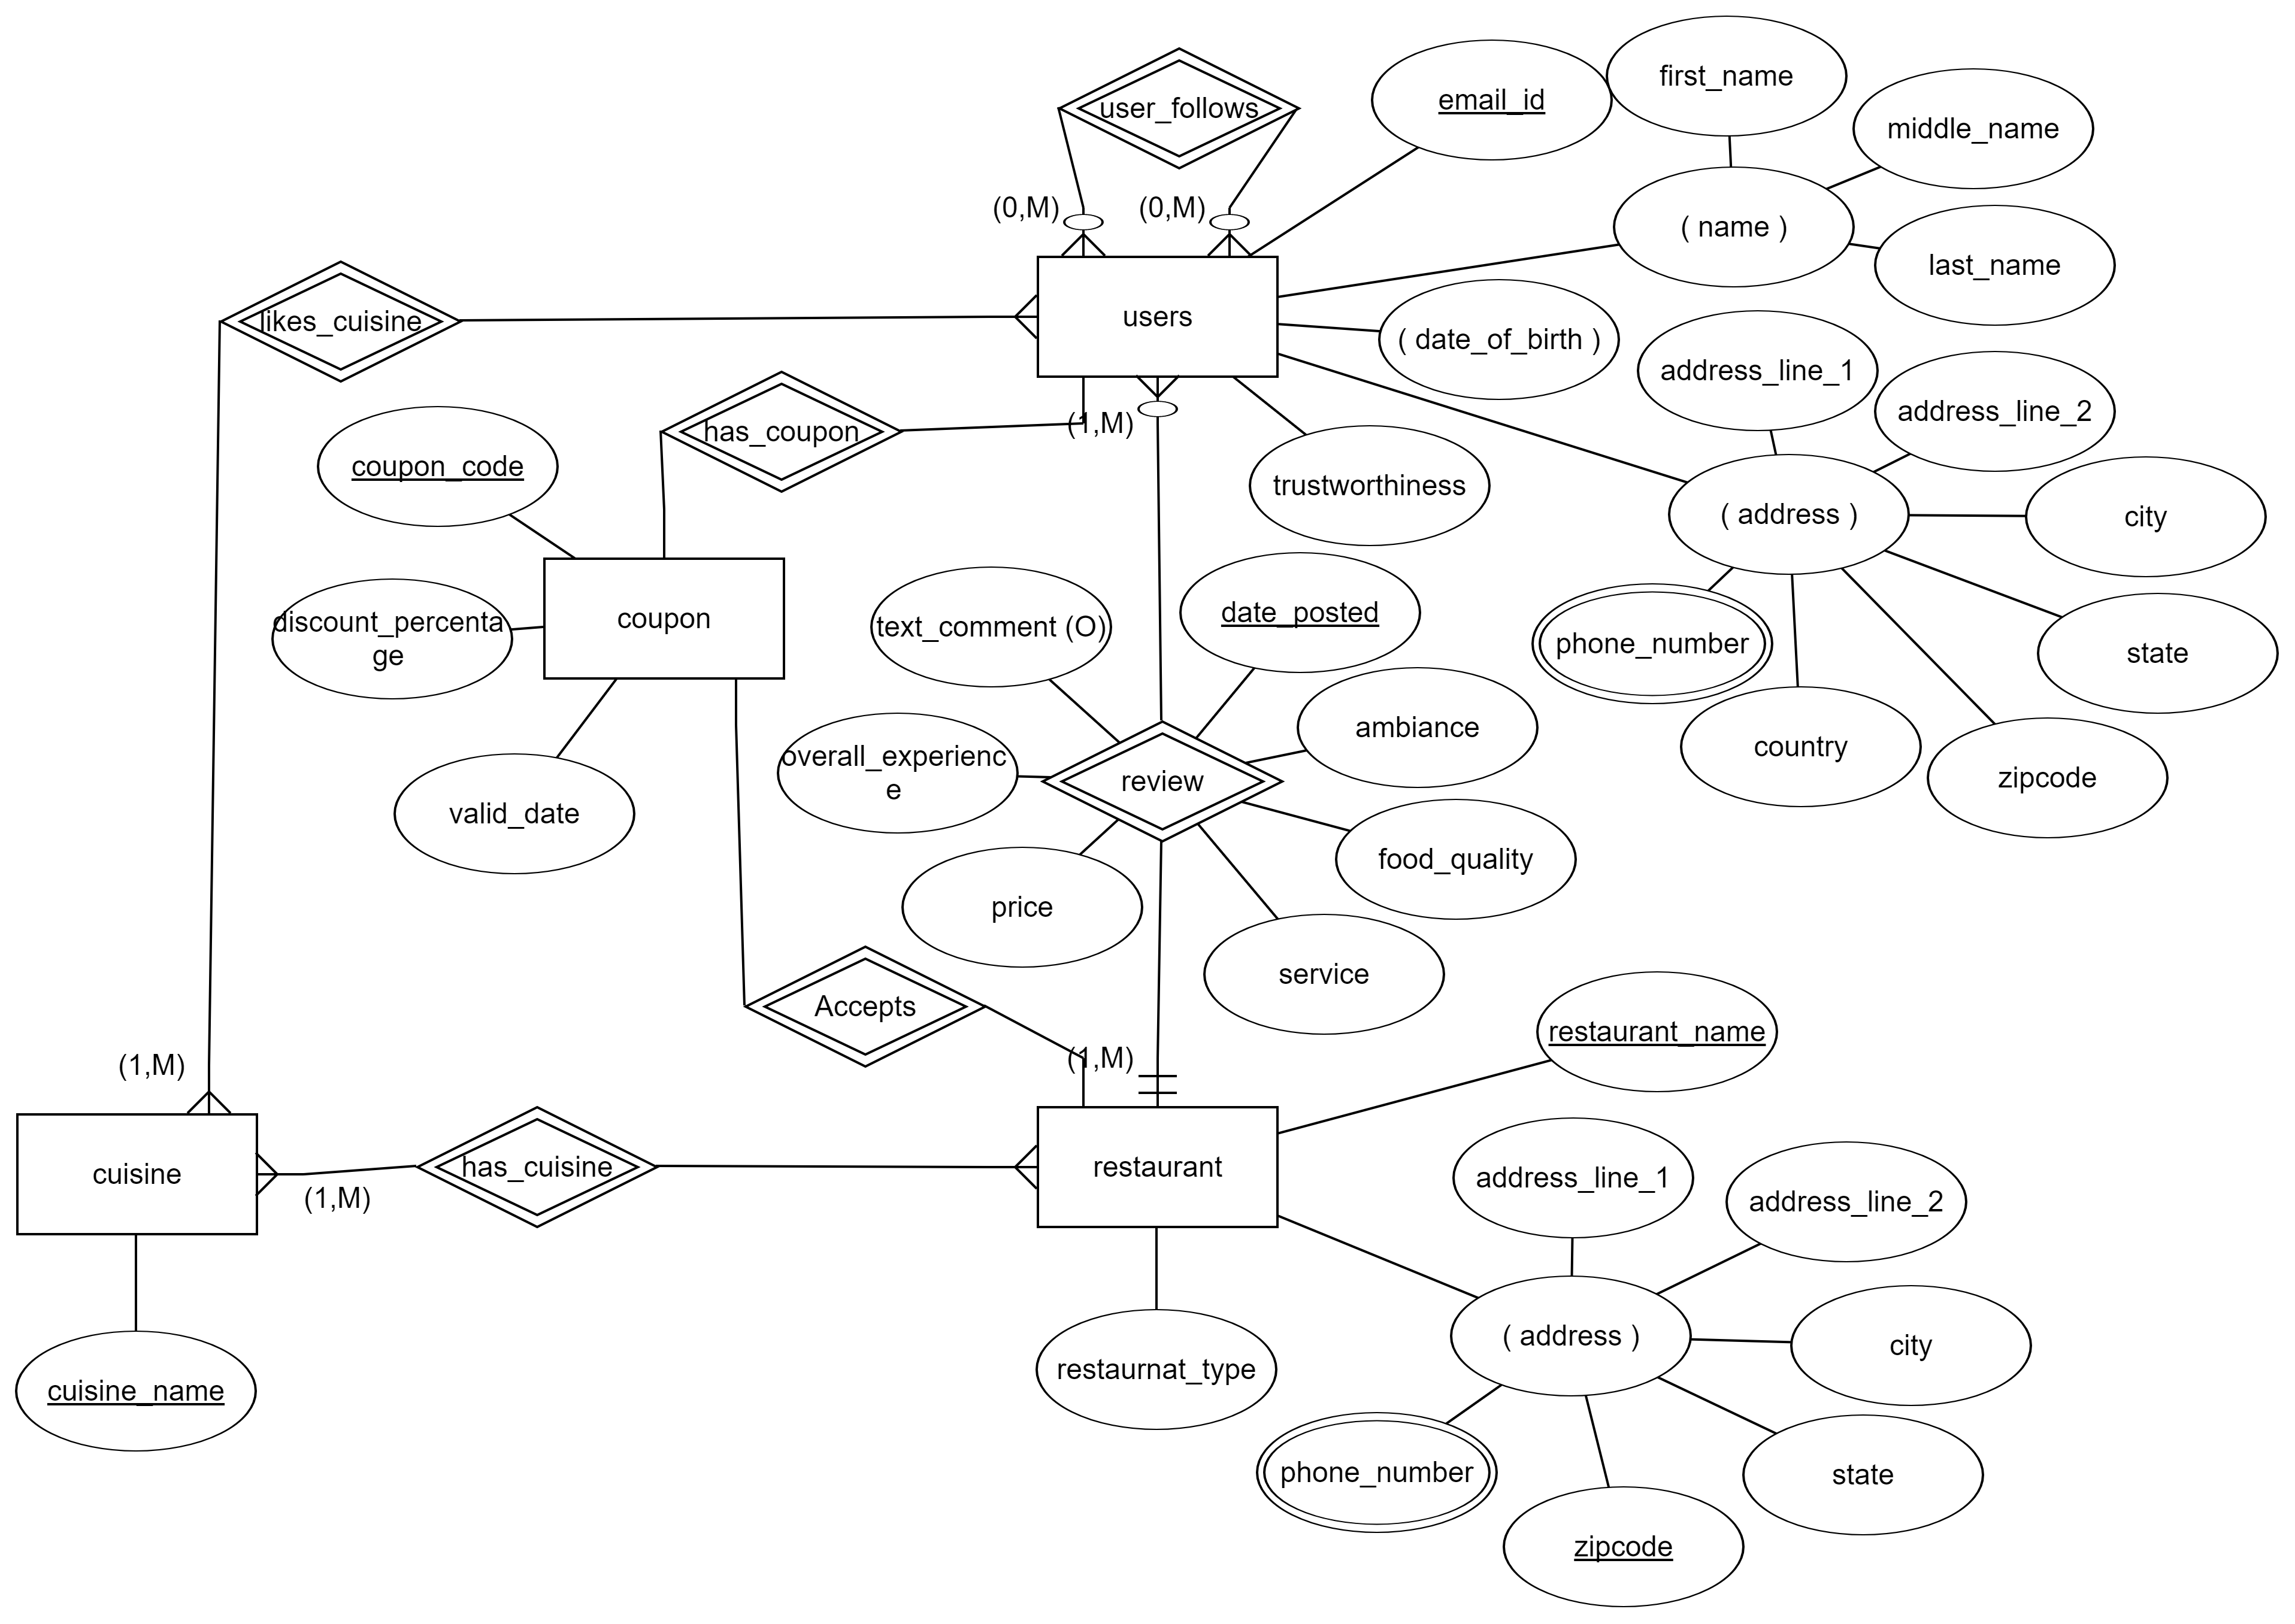
\includegraphics[scale=0.13]{er}
\end{center}
\newpage
\end{figure}
\begin{figure}[H]
\begin{center}
\caption{ER (or EER) diagram}
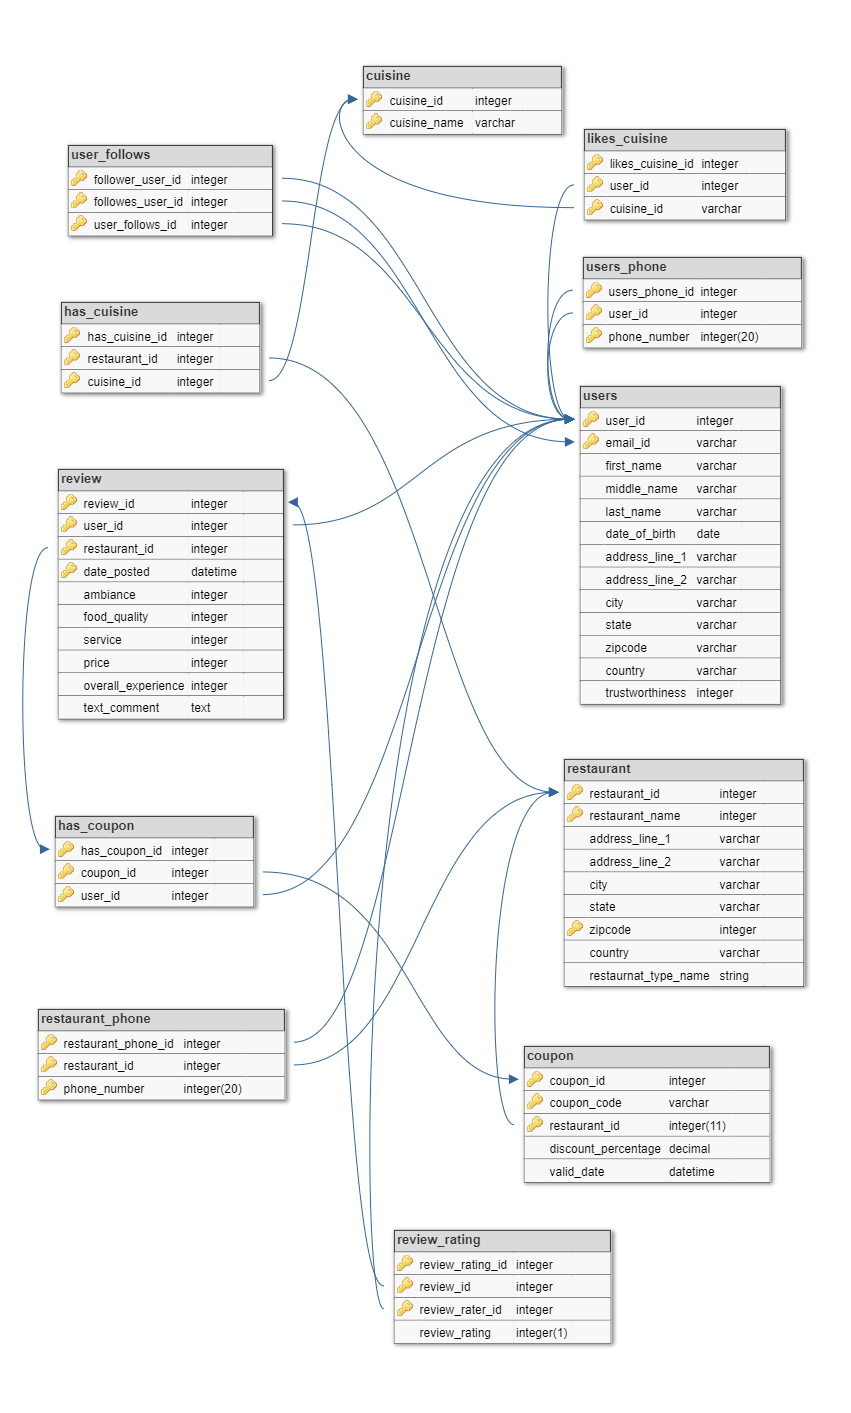
\includegraphics[scale=0.65]{rt}
\end{center}
\end{figure}
Apart from table specified in the requirement, review\_rating (user\_rating and restaurant\_rating not shown) table has been implemented in the MySQL database for trustworthiness calculation. Trustworthiness of user is derived from ratings given by other users for the reviews. Also, a separate table user\_trustworthiness table was generated later and restaurant\_rating table was also added later on.
\section*{Implementation}
Implemented restaurant recommendation database using any MySQL. Created database, tables using SQL script. Also, inserted data using a script.
into the database. Generated the fron-end using Django and Python. For connecting to MySQL database to python script, MySQLdb connector was used. For connecting to web server, Django web framework was deployed. For front-end development, HTML, Bootstrap has been used in small scale.\\\\
For average user trustworthiness:
\begin{verbatim}
SELECT users.user_id, users.first_name, users.last_name,
       AVG(review_rating.review_rating)
          FROM users, review_rating, review
               WHERE users.user_id = review.user_id 
                    AND review.review_id = review_rating.review_id
                        GROUP BY user_id;
\end{verbatim}
For finding favorite cuisine of one user:
\begin{verbatim}
SELECT users.first_name, users.middle_name, users.last_name,
       cuisine.cuisine_name FROM users, likes_cuisine, cuisine
               WHERE users.user_id = likes_cuisine.user_id 
                    AND cuisine.cuisine_id = likes_cuisine.cuisine_id
                       AND users.first_name = "Jenifer"
\end{verbatim}
For finding close restaurant restaurant recommendations with liked cuisine in same zipcode for one user:
\begin{verbatim}
SELECT users.first_name, users.last_name, restaurant.restaurant_name,
       restaurant.zipcode FROM restaurant, users, likes_cuisine,
       has_cuisine, cuisine WHERE users.user_id = likes_cuisine.user_id
           AND has_cuisine.restaurant_id = restaurant.restaurant_id 
           AND cuisine.cuisine_id = likes_cuisine.cuisine_id
           AND cuisine.cuisine_id = has_cuisine.cuisine_id
                    AND restaurant.zipcode = users.zipcode 
                    AND users.first_name = "Jenifer";
\end{verbatim}

For finding close restaurant based on food quality for one user in close proximity(same zipcode):
\begin{verbatim}
SELECT restaurant.restaurant_name, restaurant.zipcode,
       AVG(review.food_quality) FROM restaurant, review 
          WHERE review.restaurant_id = restaurant.restaurant_id
               AND restaurant.zipcode IN (SELECT zipcode FROM users
                   WHERE users.first_name = "Jenifer" 
                   AND users.last_name ="Hudson");

\end{verbatim}
\subsection*{Web Interface For Running SQL}
Developed web interface using Django open-source web framework.\\
To see search using the web interface, please install Django web framework.\\\\
Steps: 
\begin{enumerate}
\item Install pip for python if not installed already.
\item Move to python directory or scripts directory in Anaconda.
\item Please enter  -"pip install Django" for installing Django.
\end{enumerate}
To open project in web interface:
\begin{enumerate}
\item To runserver for current project go to project folder "restaurant\_recommendation" where manage.py file is located.
\item Open command prompt in the directory of manage.py and type manage.py  preceded by python.exe location and python in the following manner:
\item \path{C:\Users\Anjana\Anaconda3\python manage.py runserver
server}
\item \path{(format - >location for python.exe+python+ manage.py)}
\item To view web interface for search engine go to http://127.0.0.1:8000/
\end{enumerate}
\section*{Limitations}
The database needed more data to work well and to understand the design efficiency. Also, more informative front end can make usability efficient.
\end{document}


